\section{Exploratory Study 1}
\label{sec:ch3-s1}
This section presents our survey and the key insights that shaped the design of Study 2.

\begin{table*}[ht]
\centering
\footnotesize
\resizebox{\textwidth}{!}{
\begin{tabular}{p{1.5cm} p{6.4cm} p{6.4cm}}
\toprule
\textbf{Participant} & \textbf{Emotion-Framed Response} & \textbf{Comfort-Framed Response} \\
\midrule
P5 & 
``Stressed about my exams, but I am happy in this room. Energising, with a calm aesthetic.'' \textit{(Situated Affect)} & 
``Usually really nice and comfortably warm in here, but today a bit cold because a window was open. Lots of daylight, few noises.'' \textit{(Environmental Quality)} \\
\addlinespace
P19  & 
``I’m tired, heavy in my legs, hungry.'' \textit{(Bodily Sensation)} & 
``It's cold, so I’d like to move closer to the window and the sunlight.'' \textit{(Actions and Adjustments)} \\
\addlinespace
P188 & 
``I feel calm and relaxed. It helps that more people are working here—I don’t feel alone.'' \textit{(Social Context)} & 
``Temperature is perfect, light from glass roof, air quality seems good. Chairs and tables are comfortable.'' \textit{(Environmental Quality)} \\
\bottomrule
\end{tabular}
}
\caption{Example excerpts from our sensitising survey. While both responses describe the same moment, emotion framings often surface internal states, bodily and affective tone, and social context. Comfort framings tend to elicit descriptions of environmental qualities and adaptive strategies.}
\label{tab:s1-contrasts}
\end{table*}
\subsection{In-Situ Experience Survey}
QR codes were placed throughout the building. Occupants could scan these codes to access a short survey (in supplementary materials). The survey was a lightweight, sensitising  probe~\cite{slovak2017reflective}\footnote{We use the term sensitising probe to describe this study’s role in orienting our interpretive lens. Rather than aiming for generalisability or validation, the survey was designed to foreground experiential articulations that could inform the deeper, situated exploration in Study 2.} to explore how occupants articulate their experience when prompted from two standpoints: \textit{emotion} and \textit{comfort}. The comfort prompt aligns with traditional building-research approaches to human experience, whereas the emotion prompt introduces our AfI framing. This approach aimed to capture in-situ reflections in real time, grounded in participants’ immediate spatial and social contexts. The paired responses served as \textit{complementary elicitations}. Our aim was to sensitise ourselves to the different experiential articulations and  explore what each framing brings into view (RQ1). We treat each textual entry as a situated \textit{``snapshot of experience''}---a momentary, first-person reflection shaped by ongoing activity, environmental cues, and affective orientation. 

\subsubsection{Methodology and Data Analysis}
Data collection spanned March and June 2024 to reflect seasonal variation in environment and occupancy (weather data in supplementary materials.) The survey yielded $241$ complete responses. Since our goal was to surface commonly occurring articulations, we conducted a semantic, inductive categorisation of all responses following~\citet{braun2022conceptual}'s guidance on conceptual-level coding, appropriate for exploratory, sensitising probes~\cite{braun2022conceptual, braun2023thematic}. The analysis was conducted by the first author and reviewed with the last author. Coding was \textit{multi-label} for responses, meaning that a single response could be assigned multiple categories (see supplementary materials).

\subsection{Survey Findings}
\label{sec:ch3-s1-findings}
We developed five categories of experiences from  $241$ survey responses using semantic, inductive coding, each reflecting distinct ways of making sense of space. We describe these, compare what the two prompts foreground, and reflect on how the in-situ snapshots surface affective dimensions of experience and inform the building walk study.

\subsubsection{Categories of Experiences} The five categories of experiences are stated next: 

\paragraph{\textbf{Situated Affect – New Vocabulary}} Here, responses foreground how a space feels to be in, and how it contributes to an evolving emotional state. Participants described their emotional state in the moment, using terms like ``calm,'' ``anxious,'' or ``energised.'' Some noted affective changes underway (``getting restless,'' “starting to feel tired”), while others linked affect to environmental cues (``the light helps me stay focused,'', ``it’s cosy so I feel safe''). 

\paragraph{\textbf{Bodily Sensation}} Responses illustrate how (dis)comfort is \textit{felt through} the body, and not merely assessed cognitively. Participants described how their body physically felt in the space, referencing posture, internal states, or sensory impressions (e.g. ``the chair is hard on my back,'' ``a bit hungry,'' ``feels stuffy''). Though often linked to environmental conditions, these expressions remained first-person bodily experiences. 

\paragraph{\textbf{Environmental Quality}} This category captures describing observable environmental conditions, rather than reflecting on how those features are experienced. Participants commented on the physical attributes of the space, including classical comfort variables (temperature, light, noise, air) and spatial features (e.g. openness, layout, greenery). These descriptions framed the environment as an object of appraisal---``it’s bright,'' ``I love the plants,'' ``feels closed off''---rather than as something experienced through or with the body. 

\paragraph{\textbf{Actions and Adjustments}} This category reflects agency and interaction---whether user-initiated, imagined, or system-triggered---within a smart environment. Participants expressed interactions, intentions, or adaptive behaviours in relation to the space. Automation was mentioned (``I initiated the motion detectors here...'', ``I think it (lighting brightness) reacts to how many people are in this space'', ``blinds went down automatically'').  This included enacted responses (``I moved to a corner''), environmental (``opened the window (to let fresh air in)'', and conditional or imagined adaptations (``I’d move if it got noisier,'' ``I’d open the window but it’s stuck''). 


\subsubsection{What Each Prompt Draws Into View}
For each prompt, we analysed \textit{richness} (number of categories per response) and \textit{prevalence} (frequency of each category across responses). Emotion responses contained significantly more experiential content than comfort responses. The mean number of expression categories per response was higher for emotion $(M = 1.49)$ than for comfort $(M = 1.10)$. Nearly half of emotion responses (55.2\%) contained more than one category, compared to 21.6\% of comfort responses. This indicates that the emotion prompt elicited \emph{richer}, multidimensional articulations, combining body sensations with social context, or linking affective tone to spatial conditions and ongoing activity.

In terms of prevalence, \textit{Situated Affect} was primarily in emotion responses (67.2\%) but nearly absent in comfort responses (0.8\%). Conversely, \textit{Environmental Quality} dominated comfort responses (80.9\%) and appeared far less in emotion responses (21.2\%). \textit{Bodily Sensation} also appeared more often in emotion (32.0\%) than comfort (8.3\%), despite being central to both framings. Mentions of other occupants (\textit{Social Context}) featured more in emotion (22.8\%) than comfort (5.8\%), while adjustments or interactions with the space (\textit{Actions and Adjustments}) appeared more often in comfort (8.7\%) than emotion (6.2\%). Figure~\ref{fig:s1-prevalence} shows this distribution with with statistical evidence in the caption showing the richness of emotion responses over comfort responses.


\subsubsection{Early Evidence Through An AfI Lens}
The paired responses in this survey show that while both prompts refer to the same moment, they evoke distinct articulations of experience. \textbf{Comfort responses centre on environmental appraisal, surfacing concerns, and pointing toward small-scale adjustments. Emotion-framed entries embed affect within a broader experiential context, describing how one feels and how the space supports or misaligns with that state.} Table~\ref{tab:s1-contrasts} shows these through example excerpts. This illustrates a central tenet of AfI that experience is actively interpreted and enacted in relation to spatial, social, and temporal cues~\cite{lottridge2011affective}.  Neither framing is privileged, but each draws different dimensions of experience into focus. Together, they sensitise us to the ways in which occupants relate to smart environments. 

\begin{figure*}[ht]
\centering
\subfloat[The building walk setup for participants.  \label{fig:bw-setup}]{\includegraphics[height=6.1cm,width=0.45\textwidth]{images/study_2/setup.jpg}}
\subfloat[A session with participants engaging in a conversation moderated by the researcher.  \label{fig:bw-session}] {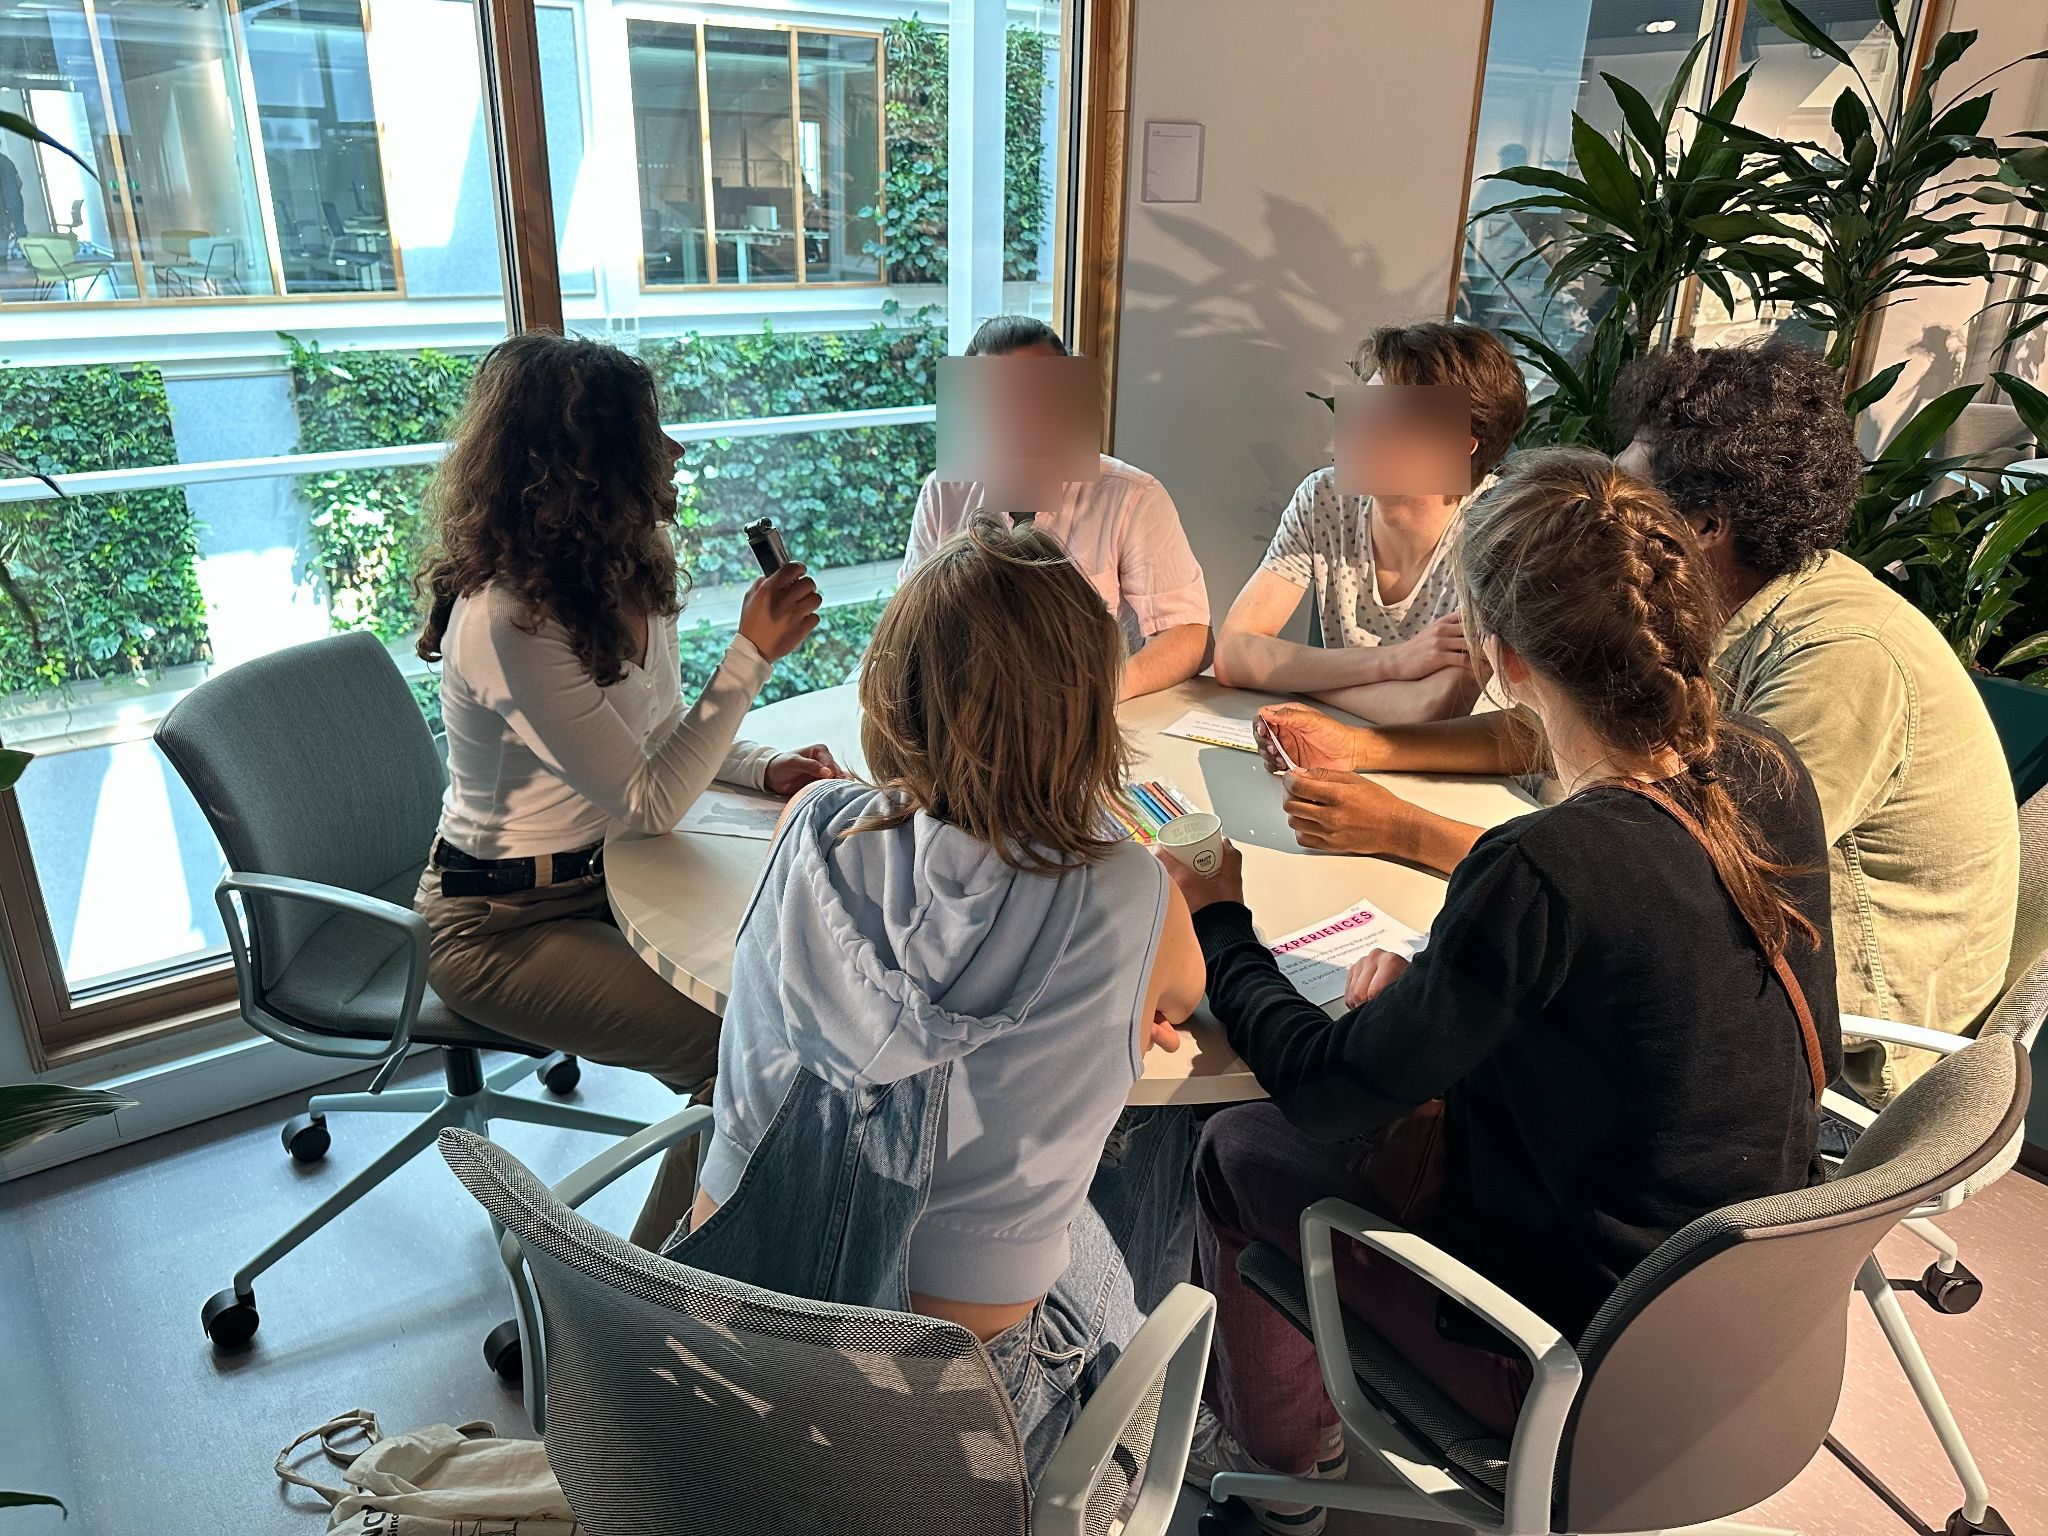
\includegraphics[width=0.456\textwidth]{images/study_2/walk.jpg}}
\caption{An overview of the building walk - (a) Setup from a session including informed consent and demographic forms, blueprints, question prompts, and body maps. (b) A session underway at a group work space. } \label{fig:s2-overview}
\Description{Two photographs documenting the building walk study. (a) A table setup showing printed informed consent and demographic forms, building floor plans, question prompt cards, and body-mapping templates prepared for participants. (b) A study session in progress, showing participants and a researcher standing and talking together in a shared indoor workspace during the building walk.}
\end{figure*}


\subsubsection*{What this foreshadows for Study 2.}
While Study 1 revealed rich, situated reflections, they remained momentary snapshots. AfI perspective calls for exploration of experiences as they develop through time~\cite{lottridge2011affective, ahmadpour2025affective}. Motivated by this, Study 2 was designed to follow occupants’ experiences across time, space, and social context---shifting focus from what people feel to how they come to feel it, and how these interpretations guide ongoing interaction.